\chapter{Modelo de Requisitos}
\label{modelo_requisitos}

En el SITEM el modelo de requisitos - junto con el de datos, es el que más importancia reviste ya que es un pilar importante para garantizar que la funcionalidad implementada es de interés para un actor específico.

\section{Modelo de Casos de Uso}
\subsection{Características Generales de los Actores}

El SITEM ofrece funcionalidad que es de interés para alguno de los siguientes actores los cuales se representan en la figura \ref{actores}:

\begin{itemize}
\item \textbf{Administrador}: Se encarga de la gestión de usuarios, el registro de nuevos subsistemas y tareas de administración tales como copias de seguridad, corrección de errores, edición de páginas, etc.
\item \textbf{Entidad de Salud}: Para la gestión especifica de información de una institución en el subsistema de Entidades de Salud. Por política general un usuario de este tipo esta confinado a la institución que crea. Para poder gestionar información de otra entidad deberá solicitar autorización a la instancia de actor dueña del registro.
\item \textbf{Servicios Médicos:} Gestiona la información de las diferentes secciones del subsistema Servicios Médicos.
\item \textbf{Especialista:} Con acceso exclusivo a su ambiente de trabajo que en la actualidad incluye registro de la hoja de vida, blog y calendario. El presente modelo de requisitos especifica algunos casos de uso para el manejo de historia clínica de pacientes y tele-consulta que están en etapa preliminar de diseño.
\item \textbf{Profesional TIC:} Actor abstracto que agrupa los actores que gestionan información en los subsistemas de: Equipos Médicos, Operadores de Telecomunicaciones, Proyectos de Telemedicina y Tecnologías de Interconexión.
\item \textbf{Usuario General:} Usuario general de consulta tiene acceso a todos los subsistemas del SITEM en modo de consulta. Puede generar informes pero no se le permite modificar ningún registro.
\item \textbf{Consultor:} Especificación del usuario general en donde además de consultar información tiene acceso a los módulo de tablas de análisis, agenda y blog.
\end{itemize}

\begin{figure}
 \centering
 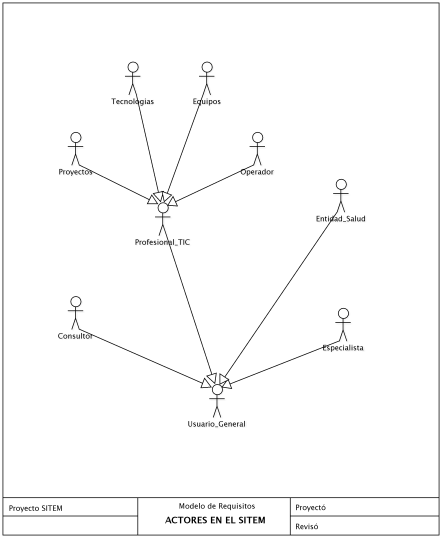
\includegraphics[width=156mm, height=182mm]{actores.png}
 \caption{Conjunto de Actores del SITEM}
 \label{actores}
\end{figure}

\subsection{Casos de Usos}
Los artefactos correspondientes a los casos de uso se han empaquetado de acuerdo al subsistema en el cual se desarrollan. En el presente documento se incluyen solo los casos que se consideran nucleares dentro de cada subsistema del SITEM. De la misma forma solo se incluyen las especificaciones de mayor relevancia e impacto.

\begin{figure}
 \centering
 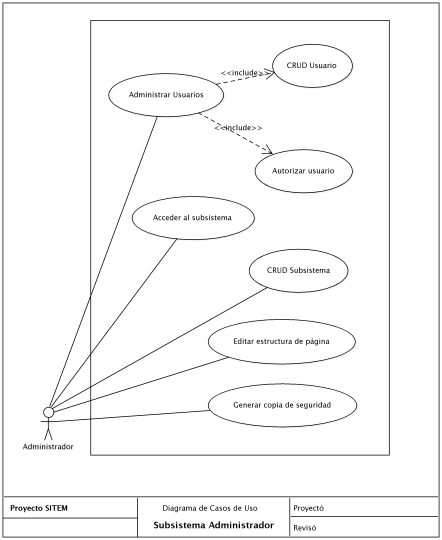
\includegraphics[width=156mm, height=182mm]{casos_admin.png}
 \caption{Casos de uso principales del Actor administrador}
 \label{casos_admin}
\end{figure}

\begin{figure}
 \centering
 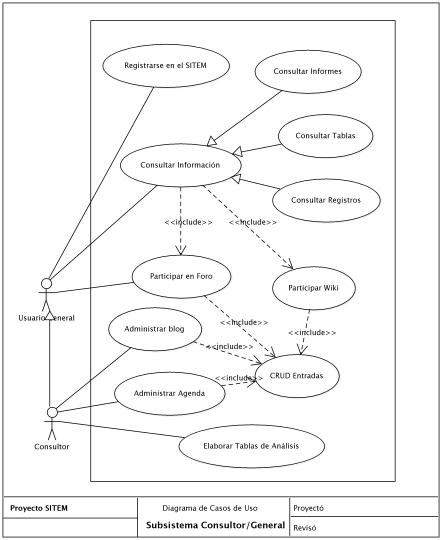
\includegraphics[width=156mm, height=182mm]{casos_consultor.png}
 \caption{Casos de uso principales del Actor Consultor/Usuario General}
 \label{casos_consultor}
\end{figure}

\begin{figure}
 \centering
 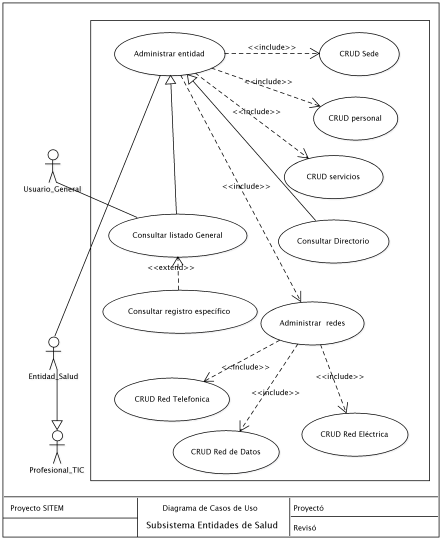
\includegraphics[width=156mm, height=182mm]{casos_entidad.png}
 \caption{Casos de uso principales del Actor Entidad de Salud}
 \label{casos_entidad}
\end{figure}

\begin{figure}
 \centering
 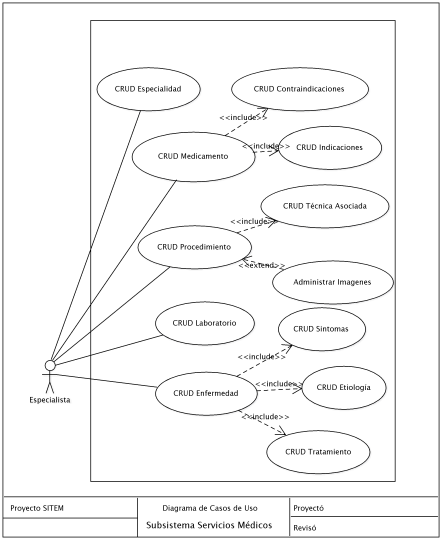
\includegraphics[width=156mm, height=182mm]{casos_servicios.png}
 \caption{Casos de uso principales del Actor Servicios Médicos}
 \label{casos_servicios}
\end{figure}

\begin{figure}
 \centering
 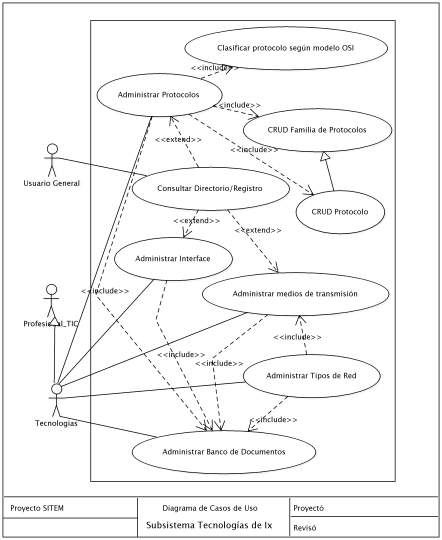
\includegraphics[width=156mm, height=182mm]{casos_tecnologias.png}
 \caption{Casos de uso principales del Actor Tecnologías de Interconexión}
 \label{casos_tecnologia}
\end{figure}

\begin{figure}
 \centering
 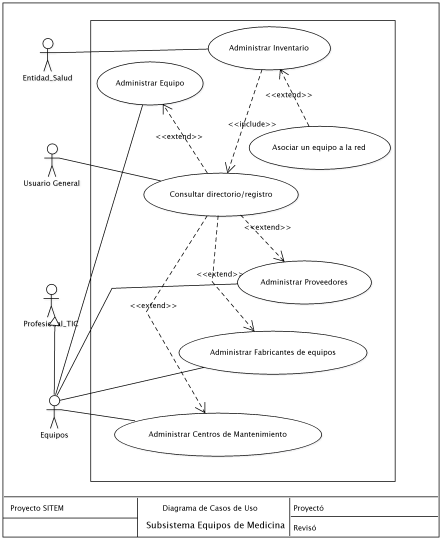
\includegraphics[width=156mm, height=182mm]{casos_equipos.png}
 \caption{Casos de uso principales en el Subsistema Equipos de Medicina}
 \label{casos_equipos}
\end{figure}

\begin{figure}
 \centering
 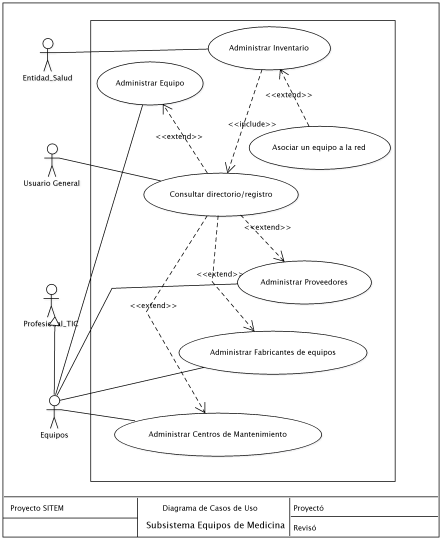
\includegraphics[width=156mm, height=182mm]{casos_equipos.png}
 \caption{Casos de uso principales en el Subsistema de Operadores de Servicios de Telecomunicaciones}
 \label{casos_telecomunicaciones}
\end{figure}
